\documentclass{patmorin}
\listfiles
\usepackage{amsthm,amsmath,graphicx}
\usepackage{array}
\usepackage{pat}
%\usepackage{coffee4}
\usepackage[letterpaper]{hyperref}
\usepackage[dvipsnames]{color}
\definecolor{linkblue}{named}{Blue}
\hypersetup{colorlinks=true, linkcolor=linkblue,  anchorcolor=linkblue,
citecolor=linkblue, filecolor=linkblue, menucolor=linkblue, pagecolor=linkblue,
urlcolor=linkblue, pdfcreator=Me, pdfproducer=Me} \setlength{\parskip}{1ex}
\usepackage{tikz}

\newcommand{\lstlabel}[1]{\label{lst:#1}}
\newcommand{\lstref}[1]{Listing~\ref{lst:#1}}
\newcommand{\Lstref}[1]{\lstref{#1}}

\DeclareMathOperator{\block}{block}
\newcommand{\naive}{na\"{\i}ve}


\newcommand{\reals}{\mathbb{R}}
\newcommand{\integers}{\mathbb{Z}}
\newcommand{\naturals}{\mathbb{N}}
\newcommand{\dist}{{d}}

\title{\MakeUppercase{New Bounds for Facial Nonrepetitive Colouring}\thanks{This research is partially funded by NSERC.}}

\author{Prosenjit Bose,\, Vida Dujmovi\'c,\, Pat Morin,\, Lucas Rioux-Maldague}



\begin{document}
\maketitle


\begin{abstract}
  We prove that the facial nonrepetitive chromatic number of any outerplanar graph is at most 11 and of any planar graph is at most 22.
\end{abstract}


\section{Introduction}
A sequence $S=s_1,s_2,\cdots,s_{2r}$, $r\ge 1$, is a \emph{repetition}
if $s_i=s_{r+i}$ for $1 \leq i \leq r$. For example, 1212 is a
repetition, while 1213 is not. Repetitions are also referred to as
\emph{squares}, since they can be written as $aa=a^2$. A \emph{block}
of a sequence $S$ is any subsequence of consecutive terms in $S$. A
sequence is \emph{nonrepetitive} (square free) if for every non-empty
block $B$
of $S$, $B$ is not a repetition. Otherwise $S$ is \emph{repetitive}. For
example, 1312124 is repetitive, as it contains the block 1212 which is a
repetition, while 123213 is nonrepetitive as it contains no such block.
It is easy to see that no sequence of length greater than 3 on two symbols
can be nonrepetitive. A result by Axel Thue in 1906 states
that nonrepetitive sequences of arbitrary length can be created using
three symbols \cite{thue1906uber}. 

A variant of this problem concerning graphs was proposed by Alon,
Grytczuk, Ha{\l}uszczak and Riordan in 2002 \cite{alon2002nonrepetitive}.
A nonrepetitive (vertex) colouring of a graph $G$ is an assignment
of colours to $G$'s vertices such that, for every path $P$ in $G$,
the sequence of colours of vertices in $P$ is not a repetition.
The \emph{nonrepetitive chromatic number} of $G$, denoted $\pi(G)$,
is the minimum number of colours required in a nonrepetitive
colouring of $G$.  Nonrepetitive graph colouring has received much
attention \cite{barat2013facial, barat2007square, barat2008note,
brevsar2007nonrepetitive, currie2002cycle18, dujmovic2012planarlogn,
dujmovic2011nonrepetitive, fiorenzi2011thue, gagol2016pathwidth,
gonccalves2014entropy,
grytczuk2007nonrepetitivesurvey, grytczuk2007nonrepetitive,
grytczuk2013new, harant2012nonrepetitive, kozik2013nonrepetitive,
kundgen2008nonrepetitive, pezarski2009non, schreyer2012facial,
schreyer2013total}.

A well-known conjecture in this area, due to Alon et al
\cite{alon2002nonrepetitive}, is that there exists a constant
$K$ such that $\pi(G) \leq K$ for any planar graph $G$.
The current best upper bound for $n$-vertex planar graphs is
$O(\log n)$ \cite{dujmovic2012planarlogn}. No planar graph
with nonrepetitive chromatic number greater than 11 is known
\cite[Appendix~A]{dujmovic2012planarlogn}.

More is known about the \emph{facial} version of the problem for embedded
planar graphs.  Harant and Jendrol \cite{harant2012nonrepetitive} asked
if every planar graph can be coloured with a constant number of colours
such that every \emph{facial} path\footnote{A facial path is a path
that is a subsequence of a facial walk; see \secref{preliminaries}.} is
nonrepetitively coloured.  Barat and Czap \cite{barat2007square} answered
this question in the affirmative with the constant $24$.  We reduce this
bound to 22 by proving a bound of 11 for facial nonrepetitive colouring
of outerplane graphs.

\subsection{Related Work}

\paragraph{Nonrepetitive Colouring.}
It is known that some families of graphs have bounded repetitive chromatic
number.  In their original work, Alon et al \cite{alon2002nonrepetitive}
showed that $\pi(G) = O(\Delta^2)$ if $G$ has maximum degree
$\Delta$ and that there are are graphs of maximum degree $\Delta$
with nonrepetitive chromatic number $\Omega(\Delta^2/\log \Delta)$.
The constants in the $O(\Delta^2)$ upper bound have been steadily
improved \cite{dujmovic2011nonrepetitive,grytczuk2007nonrepetitive,
grytczuk2007nonrepetitivesurvey,harant2012nonrepetitive}.

K{\"u}ndgen and Pelsmajer \cite{kundgen2008nonrepetitive} showed that
$\pi(G)\le 12$ if $G$ is outerplanar and, more generally, $\pi(G)\le 4^t$
if $G$ has treewidth at most $t$. The latter bound is tight if $t=1$
(trees), but it is not known if it is tight for other values of $t$. Even
the upper bound of 12 for outerplanar graphs is not known to be tight,
as no outerplanar graph with nonrepetititive chromatic number greater
than 7 is known \cite{barat2007square}.

\paragraph{Facial Nonrepetitive Colouring.}

Facial nonrepetitive colouring was first considered by Havet et al
\cite{havet2011facial}, who studied the edge-colouring variant of
the problem.  In this setting, they were able to show that the edges
of any plane graph can 8-coloured so that every facial trail\footnote{A
\emph{facial trail} is a subsequence of the edges traversed during the
boundary walk of a face.} is coloured nonrepetitively. 

For the vertex-colouring version we study, Harant and Jendrol prove
that $\pi_f(G)=O(\log\Delta)$ if $G$ is a plane graph of maximum
degree $\Delta$ and that $\pi_f(G)\le 16$ if $G$ is a Hamiltonian
plane graph.  They also conjectured that $\pi_f(G)=O(1)$ when $G$
is any plane graph.  This latter conjecture was confirmed by Barat
and Czap \cite{barat2007square}, who showed that $\pi_f(G)\le 24$ for
any plane graph $G$.  The best lower bounds for facial nonrepetitive
chromatic numbers are 5 for plane graphs and 4 for outerplane graphs
\cite{barat2013facial}


%
%In this paper, we consider a variation of Thue colourings
%for plane graphs in which we only require facial paths to be
%nonrepetitive.
%A \emph{plane graph} $G$ is a fixed embedding of a graph in the plane such that its edges intersect only at their endpoints. An \emph{outerplane} graph $G$ is a plane graph such that all the vertices of $G$ are adjacent to the outside face of $G$. 
%A \emph{closed walk} in a graph $G$ is a sequence of vertices $v_0,\ldots,v_{\ell-1}$ such that, for every $i\in\{0,\ldots,\ell-1\}$ the edge $v_iv_{(i+1)\bmod \ell}$ is in $E(G)$.
%A \emph{facial walk} in a plane graph $G$ is a closed walk
%$v_0,\ldots,v_{\ell-1}$ such that, for every $i\in\{0,\ldots,\ell-1\}$,
%the edges $v_{(i-1)\bmod \ell} v_i$ and $v_iv_{(i+1)\bmod\ell}$ occur
%consecutively in the counterclockwise cyclic ordering of the edges
%incident to $v_i$ in the embedding of $G$.
%A \emph{facial path} is a contiguous subsequence of a facial walk that
%is a path in $G$.
 
%
%An edge-colouring variant of facial non-repetitive colouring was first introduced
%by Havet et al. \cite{havet2011facial}, then Harant and Jendrol
%\cite{harant2012nonrepetitive} followed up with results for the
%vertex-colouring setting we study here. A 
%\emph{nonrepetitive facial $k$-colouring} is a vertex
%$k$-colouring in which for every facial path $(v_1,\cdots,v_n)$ in $G$,
%the sequence $c(v_1),\cdots, c(v_n)$ is nonrepetitive. The \emph{facial
%Thue chromatic number} of a graph $G$, denoted $\pi_f(G)$, is the least
%$k$ for which a nonrepetitive facial $k$-colouring of $G$ exists. As with
%Conjecture \ref{conj:planarConstant} for the Thue chromatic number, it
%was also conjectured by Harant and Jendrol \cite{harant2012nonrepetitive}
%that there exists a constant $K$ such that $\pi_f(G) \leq K$ for any plane
%graph $G$. This conjecture was confirmed with $K=24$ by Barat and Czap
%\cite{barat2013facial}, and with smaller values of $K$ when restricted
%to some families of 2-connected\footnote{A graph is $k$-connected if
%it contains more than $k$ vertices and has no vertex cut of size less
%than $k$.} plane graphs such as Halin graphs ($K=??$) and Hamiltonian plane
%graphs ($K=16$) \cite{harant2012nonrepetitive}. Any nonrepetitive colouring is
%also a facial nonrepetitive colouring so we have that $\pi_f(G) \leq
%\pi(G)$. The best lower bound for the facial Thue chromatic number is
%5 for plane graphs and 4 for outerplane graphs \cite{barat2013facial}.
%
%TODO: Ask Lucas where Halin graphs come from?
%
%In the next sections, we prove tighter bounds for the facial Thue chromatic number of outerplane and plane graphs. Our technique consists in finding a \emph{blocking set}, from which we construct a \emph{blocking graph}. The blocking set is such that its removal from the outerplane graph results in a forest, for which a nonrepetitive 4-colouring exists. We show that a facial nonrepetitive colouring of any outerplane graph can be obtained by combining this colouring of a forest and a facial nonrepetitive colouring of the blocking graph.
%We then proceed to show how to find a nonrepetitive colouring on at most 7 colours of the blocking graph. Although it seems hard --- if not impossible --- to find a such a colouring if the blocking graph contains odd cycles, we show that this is feasible if all cycles are even, and that it is possible to select the blocking set as such.
%
%From this technique, we show that the facial Thue chromatic number of a plane graph is bounded by 22, by 11 for outerplane graphs and by 7 for 2-connected outerplane graphs. Let $G$ be a graph and $H$ be a subgraph of $G$. $G[H]$ is the subgraph of $G$ induced by $V(H)$. Let $G$ be a plane graph. $\wdual{G}$ is the \emph{weak dual} of $G$, the subgraph of the dual of $G$ whose vertices correspond to the bounded faces of the $G$. A $k$-connected component of $G$ is a maximal induced subgraph $H$ of $G$ that is $k$-connected.
%

\section{Preliminary Results and Definitions}
\seclabel{preliminaries}

All graphs we consider are undirected, but not necessarily simple.  For a
graph, $G$, we use the notations $V(G)$ and $E(G)$ to denote $G$'s vertex
and edge sets, respectively. For $S\subset V(G)$, $G[S]$ denotes the
subgraph of $G$ induced by the vertices in $S$ and $G-S=G[V(G)\setminus
S]$.

A graph is \emph{$k$-connected} if it contains more than $k$ vertices
and has no vertex cut of size less than $k$.  A \emph{$k$-connected
component} of a graph $G$ is a maximal subset of vertices $G$ that
induces a $k$-connected subgraph.

A \emph{bridge} in a graph $G$ is an edge whose removal increases the
number of connected components in $G$.  A graph is \emph{bridgeless}
if it has no bridges.

A \emph{plane graph} $G$ is a fixed embedding of a graph in the plane such
that its edges intersect only at their endpoints. An \emph{outerplane}
graph $G$ is a plane graph such that all the vertices of $G$ are incident
on the outer face of $G$. A \emph{chord} in an outerplane graph is
an edge that is not incident to the outer face. A \emph{cactus graph}
is an outerplane graph with no chords.  An \emph{ear} in an outerplane
graph is an inner face that is incident to exactly one chord. An ear is
\emph{triangular} if it has exactly three vertices.

A \emph{closed walk} in a graph $G$ is a sequence of vertices
$v_0,\ldots,v_{\ell-1}$ such that, for every $i\in\{0,\ldots,\ell-1\}$
the edge $v_iv_{(i+1)\bmod \ell}$ is in $E(G)$.
A \emph{facial walk} in a plane graph $G$ is a closed walk
$v_0,\ldots,v_{\ell-1}$ such that, for every $i\in\{0,\ldots,\ell-1\}$,
the edges $v_{(i-1)\bmod \ell} v_i$ and $v_iv_{(i+1)\bmod\ell}$ occur
consecutively in the counterclockwise cyclic ordering of the edges
incident to $v_i$ in the embedding of $G$.  A \emph{facial path} is a
contiguous subsequence of a facial walk that is a path in $G$.

Before proceeding with our results, we will introduce a helper lemma
due to Havet et al.~\cite{havet2011facial} and two major results which
will be used throughout the paper. The helper lemma provides a way to
interlace nonrepetitive sequences.

\begin{lem}[Havet et al. \cite{havet2011facial}]\lemlabel{interleave}
  Let $B=B_1,B_2,\ldots,B_k$ be a nonrepetitive sequence over an alphabet
  $\mathcal{B}$ in which each $B_i$ has size at least 1. For each $i
  \in \{0,\ldots,k\}$, let $A_i$ be a (possibly empty) nonrepetitive
  sequence over an alphabet $\mathcal{A}$ with $\mathcal{B} \cap
  \mathcal{A} = \emptyset$. Then $S = A_0, B_1, A_1, \ldots, B_k, A_k$
  is a nonrepetitive sequence.
\end{lem}

We will require two results about the nonrepetitive chromatic number of
trees and cycles:

\begin{thm}[Alon et al. \cite{alon2002nonrepetitive}]\thmlabel{tree}
  For every tree, $T$, $\pi(T) \leq 4$.
\end{thm}

\begin{thm}[Currie \cite{currie2002cycle18}]\thmlabel{cycle}
  For every $n>2$, the cycle $C_n$ on $n$ vertices has
  \[
  \pi(C_n) = \begin{cases}
              4 & \text{ if } n \in \{5,7,9,10,14,17\} \\
              3 & \text{ otherwise. }
             \end{cases}
  \]
\end{thm}

\section{Outerplane Graphs}

We begin with a simple lemma that allows us to focus, when convenient,
on simple outerplane graphs.

\begin{lem}\lemlabel{non-simple}
  Let $G$ be a simple outerplane graph and let $G'$ be an outerplane graph obtained by adding parallel edge and/or loops to $G$.  Then $\pi_f(G')\le\pi_f(G)$.
\end{lem}

\begin{proof}
   We argue that any facial path in $G'$ is also a facial path in $G$.
   Therefore, by facially nonrepetitively colouring $G$, we obtain a facial
   nonrepetitive colouring of $G'$.

   First, note that no facial path uses a loop, so the addition of
   loops does not introduce new facial paths in $G'$.  When an edge
   $e'$ is added parallel to an existing edge $e$ of $G$, the union
   of the embeddings of $e$ and $e'$ form a Jordan curve that does not
   contain any vertices of $G$ (since we require $G'$ to be outerplane).
   This implies that any facial path in $G'$ that uses the new edge $e'$
   exists in $G$ as a facial path that uses the edge $e$.
\end{proof}

Let $G$ be an outerplane graph. A \emph{blocking set} of $G$ is a set
of vertices $B \subseteq V(G)$ such that for each 2-connected component
$H$ of $G$, $H-B$ is a tree and for each inner face $F$,
$V(F) \setminus B \ne \emptyset$.  See Figure \ref{fig:blocking-set}
for an example of a blocking set.

\begin{figure}
  \begin{center}
     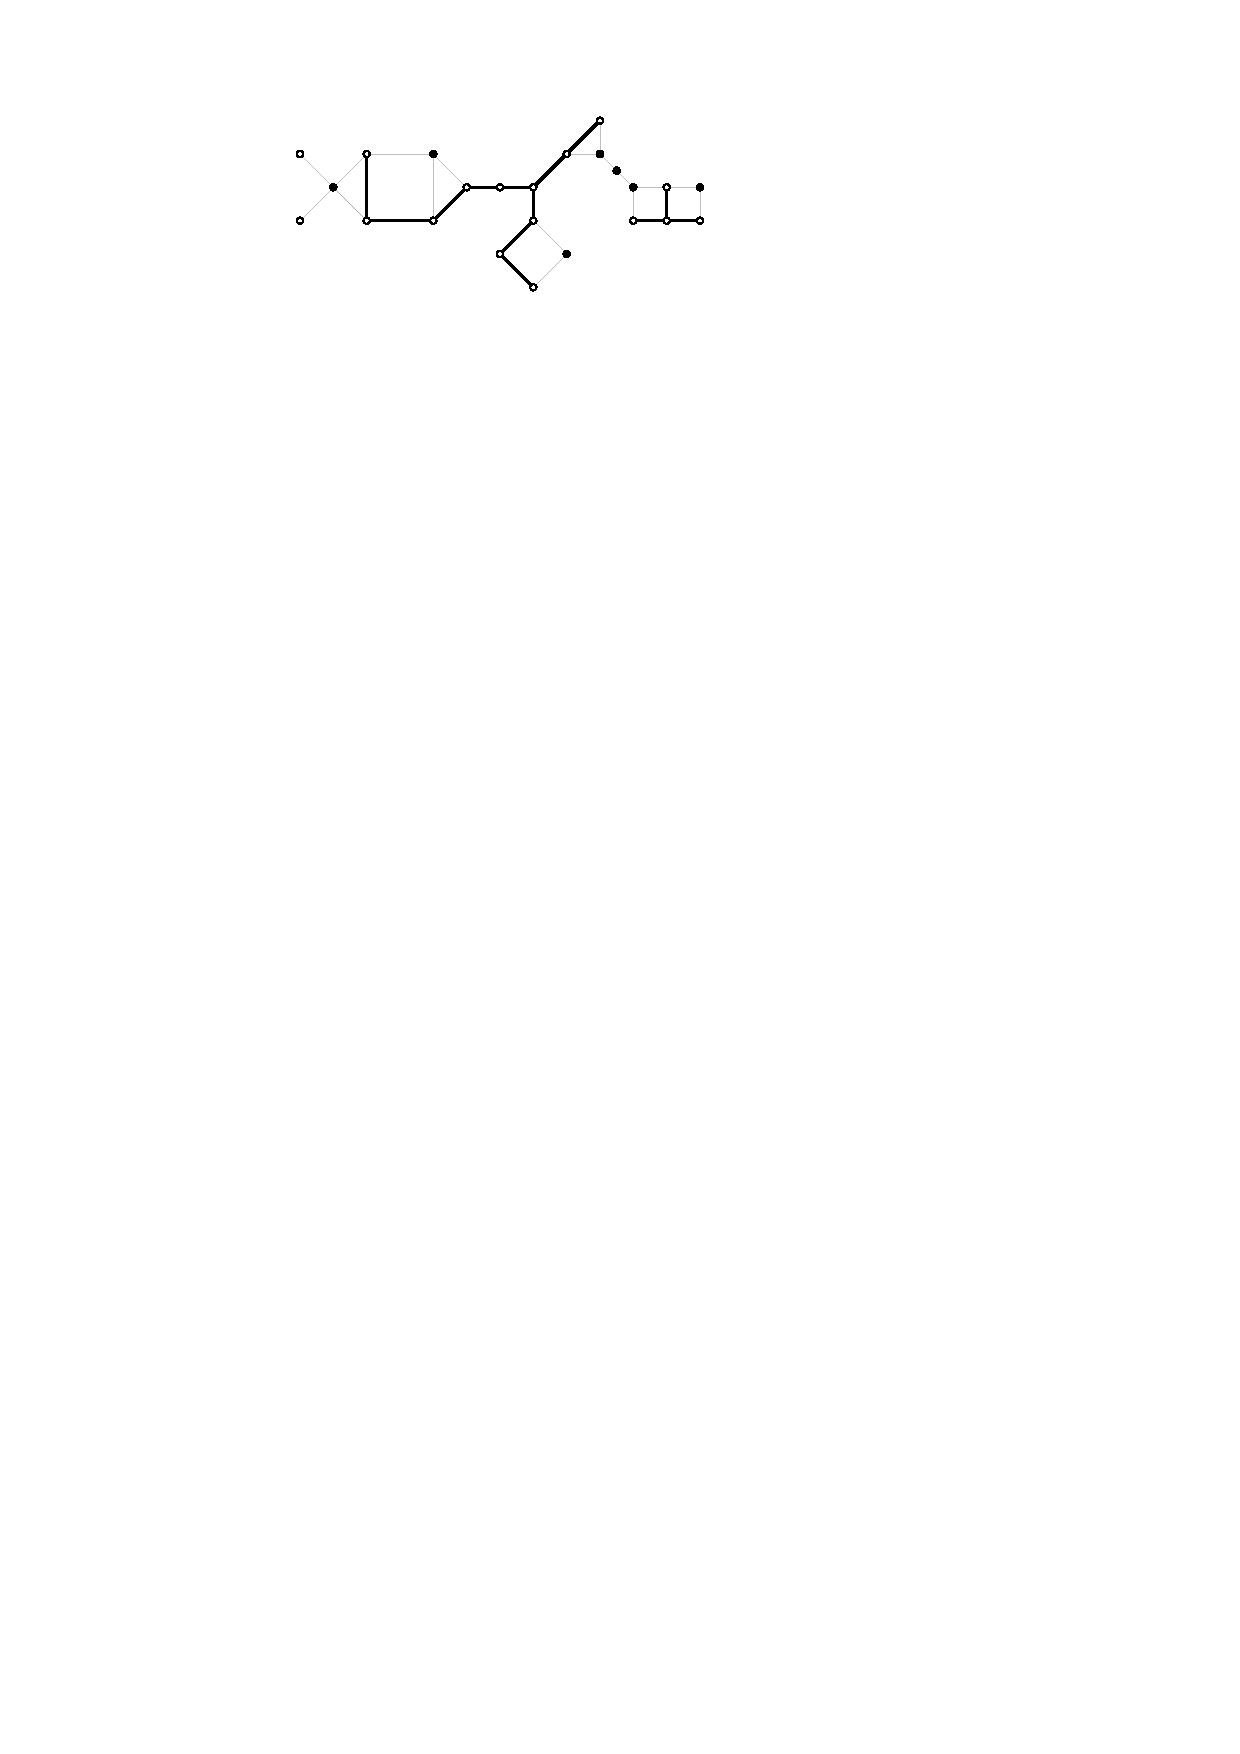
\includegraphics{figs/blocking-set-1}
  \end{center}
  \caption{The blocking set of an outerplane graph (in black).}
  \figlabel{blocking-set}
\end{figure}

The definition of a blocking set is subtle and implies three properties
that we will use throughout.   

\begin{obs}\obslabel{no-chords}
   For any blocking set $B$ of $G$, $B$ does not include both endpoints
   of any chord of $G$.
\end{obs}

\begin{obs}\obslabel{consecutive}
   For any blocking set $B$ of $G$ and any inner face $F$ of $G$, the
   vertices of $V(F)\cap B$ occur consecutively on the boundary of $F$.
\end{obs}

\begin{obs}\obslabel{non-empty-path}
  For every inner face $F$ of $G$, $F-B$ is a non-empty path.
\end{obs}


\begin{lem}\lemlabel{biconnected}
  For every biconnected outerplane graph, $G$, and any vertex $v\in
  V(G)$, there exists a blocking set $B$ of $G$ such that $v\in B$ and,
  for each inner face $F$ of $G$, $|B\cap V(F)|=1$.
\end{lem}

\begin{proof}
  The proof is by induction on the number of inner faces.  If $G$ has
  only face, we take $B=\{v\}$.  Otherwise, select some ear, $F$ of $G$
  whose chord is $uw$ and such that $v\not\in V(F)\setminus\{u,w\}$.
  Let $G'=G-(V(F)\setminus\{u,w\})$.  The graph $G'$ has one less inner
  face than $G$ so, by induction, it has a blocking set $B'$ that satisfies
  the conditions of the lemma.  There are two cases to consider:
  \begin{enumerate}
    \item If one of $u$ or $w$ is in $B'$ then we take $B=B'$ to obtain
      a blocking set that satisifes the conditions of the lemma.

    \item Otherwise, let $x$ be any vertex in $V(F)\setminus\{u,w\}$ and
      take $B=B'\cup\{x\}$ to obtain a blocking set that satisifes the
      conditions of the lemma. \qedhere
  \end{enumerate}
\end{proof}

\Lemref{biconnected} allows us to prescribe that a particular vertex
$v$ be included in the blocking set, but it will also be convenient to
exclude a particular vertex $v$ by using \lemref{biconnected} to force
the inclusion of $v$'s neighbour on the outer face (which is also on
some inner face with $v$).

\begin{cor}\corlabel{biconnected-out}
  For every biconnected outerplane graph, $G$, and any vertex $v\in
  V(G)$, there exists a blocking set $B$ of $G$ such that $v\not\in B$ and,
  for each inner face $F$ of $G$, $|B\cap V(F)|=1$.
\end{cor}

At this point we pause to sketch how \lemref{biconnected}
can already be used to give an upper-bound of 8 on the facial
nonrepetitive chromatic number of biconnected outerplane graphs.  For a
biconnected outerplane graph, $G$, we take a blocking set $B$ of $G$
using \lemref{biconnected}.  By \thmref{tree}, we can nonrepetitively
4-colour the tree $T=G-B$ using the colours $\{1,2,3,4\}$, so
what remains is to assign colours to the vertices in $B$.  To do this,
we use \thmref{cycle} to nonrepetitively 4-color the cycle, $C$, that
contains the vertices of $B$ in the order they appear on the outer face
of $G$ using the colours $\{5,6,7,8\}$.  We claim that the resulting
8-colouring of $G$ is facially nonrepetitive.  No facial path on an
inner face is coloured repetitively since each such facial path is also
either present in the tree $T$ or it contains exactly one vertex of $B$.
No facial path on the outer face is coloured repetitively since it is
obtained by interleaving a nonrepetitive sequence of colours in $C$
with nonrepetive sequences taken from $T$; by \lemref{interleave},
a sequence obtained in this way is nonrepetitive.

In \appref{biconnected}, we show that the preceding argument can be
improved to give a bound of 7 on the facial nonrepetitive chromatic
number of biconnected outerplane graphs. This is just a matter of adding
vertices to the blocking set so that the cycle $C$ does not have length
in $\{5,7,9,10,14,17\}$, so that it can nonrepetitively 3-coloured.

\subsection{The Blocking Graph}


The \emph{blocking graph}, $\block_B(G)$, of $G$ for a blocking set $B$ is
the graph whose vertex set is $B$ and whose edges are defined as follows:
Begin with the facial walk $W$ on the outer face of $G$. Remove every
vertex not in $B$ from $W$ to obtain a cyclic sequence $W'$ of vertices
in $B$. For each consecutive pair of vertices $uw$ in $W'$ we add the
edge $uw$ to $\block_B(G)$.  This naturally defines the embedding of the
blocking graph. See \figref{blocking-graph} for an example.   Note that
$\block_B(G)$ is a plane graph that is not necessarily simple graph;
it may contain parallel edges (cycles of length two) and self-loops
(cycles of length one).

\begin{figure}
  \begin{center}
     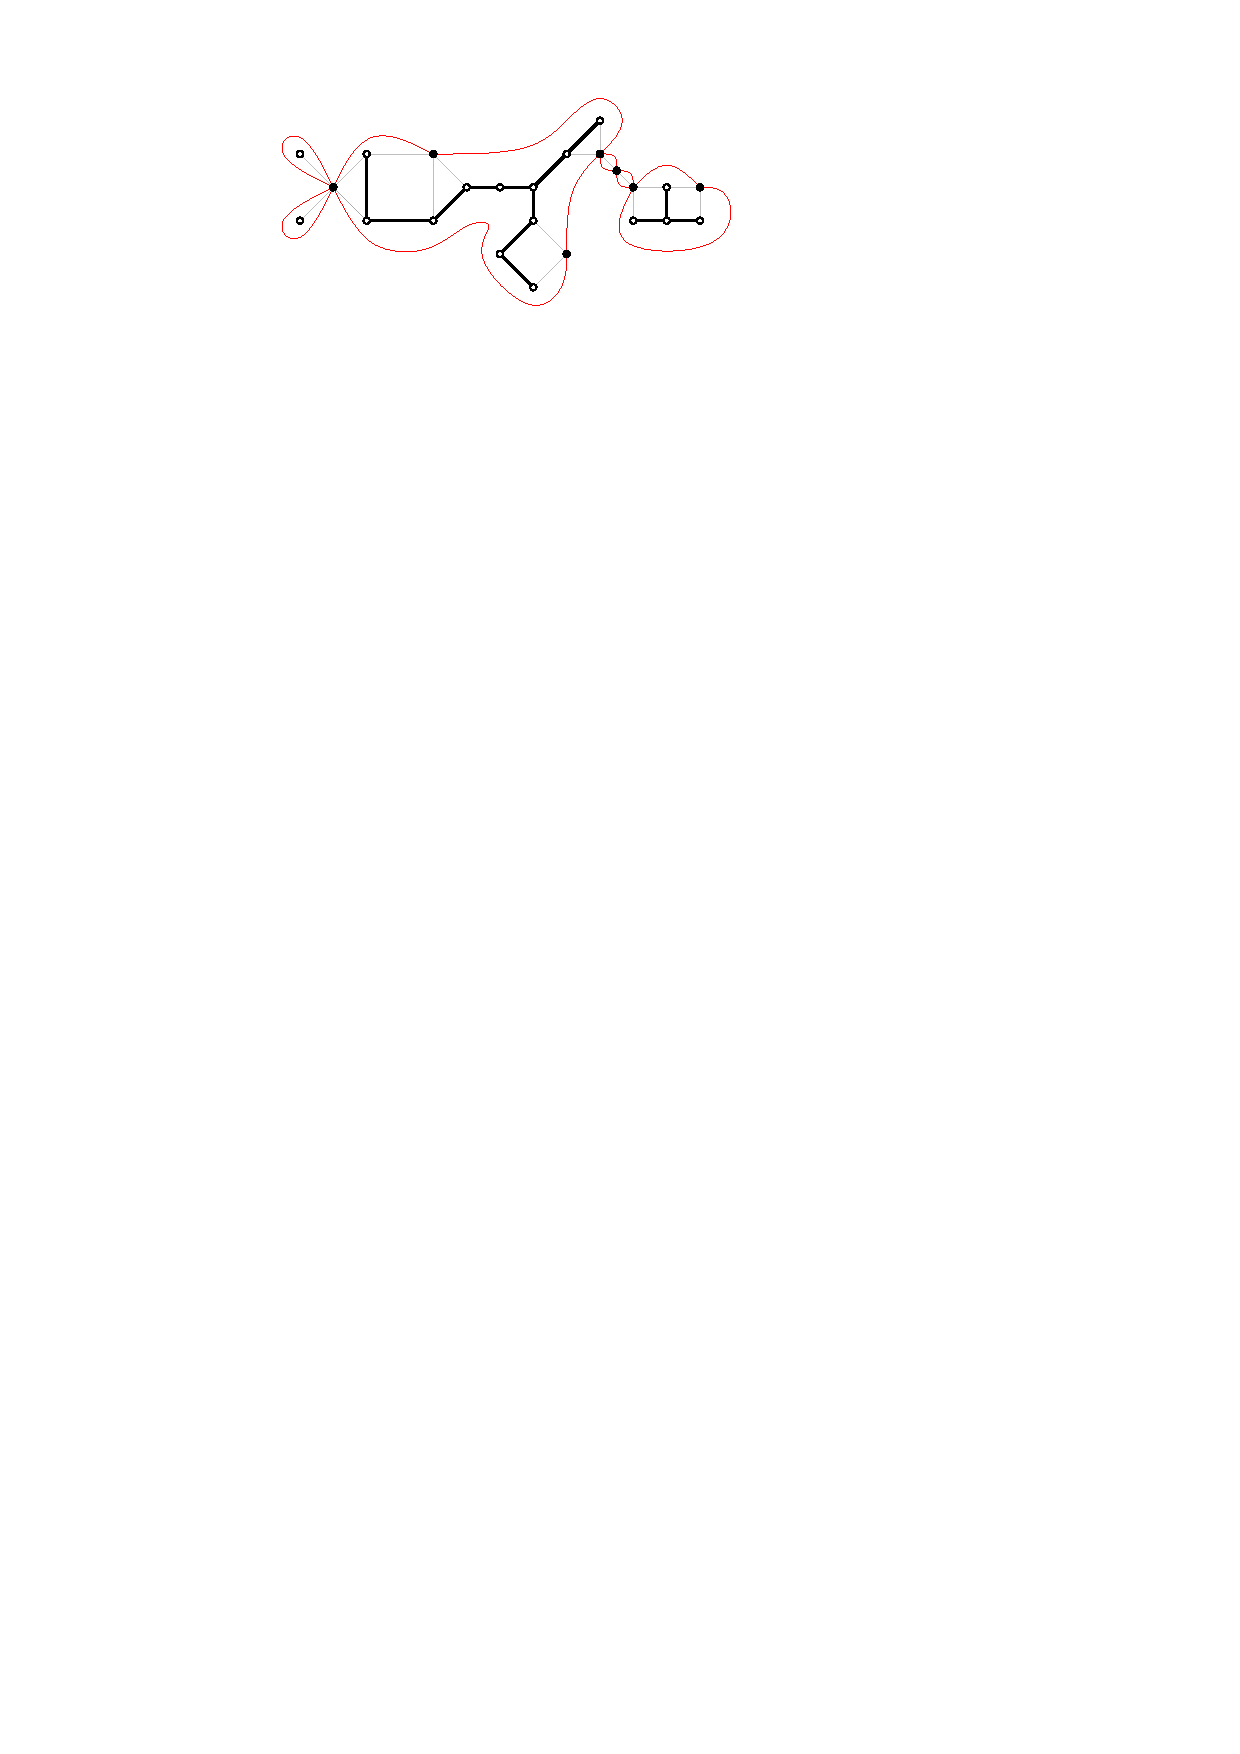
\includegraphics{figs/blocking-set-2}
  \end{center}
  \caption{The blocking graph (edges in red) associated with a blocking set (vertices in black).}
  \figlabel{blocking-graph}
\end{figure}

The fact that a blocking set does not contain both endpoints of any
chord of $G$ (\obsref{no-chords}) implies the following observation:

\begin{obs}\obslabel{cactus}
   For every outerplane graph $G$ and any blocking set $B$ of $G$,
   the blocking graph $\block_B(G)$ is a bridgeless cactus graph.
\end{obs}

\begin{obs}\obslabel{shit0}
For every outerplane graph $G$, any blocking set $B$ of $G$ and any
facial path $P$ on the outer face of  $G$, the subsequence of $P$
containing only the vertices of $B$ is a (outer) facial path in $\block_B(G)$.
\end{obs}

\begin{obs}\obslabel{shit}
For every outerplane graph $G$, any blocking set $B$ of $G$ and any
inner face $F$ of $G$, $G[V(F)\cap B]$ is a path that is a facial path (on
some inner face)  in $\block_B(G)$.
\end{obs}

In the previous section, we sketched a proof of an upper bound of 8 on
the facial chromatic number of biconnected outerplane graphs.  This proof
works by nonrepetitively 4-colouring the tree, $G-B$, obtained after
removing the blocking set and then nonrepetiviely 4-colouring a cycle,
$C$, of vertices in the blocking set.  This cycle, $C$, is actually
the blocking graph, $\block_B(G)$.  The following lemma shows that
this strategy generalizes to the situation where we can find a facial
nonrepetitive colouring of $\block_B(G)$ with few colours.

\begin{lem}\lemlabel{hitting_plus_four}\lemlabel{k-plus-four}
  Let $G$ be an outerplane graph and $B$ be a blocking set of $G$. If
  there exists a facial nonrepetitive $k$-colouring of (the outer 
  face of) $\block_{B}(G)$, then there exists a facial nonrepetitive
  $(4+k)$-colouring of $G$.
\end{lem}

\begin{proof}
By \thmref{tree} we can colour $G-B$ nonrepetitively using colours
$\{1,2,3,4\}$. By the assumption we can colour  facially
nonrepetitively $\block_{B}(G)$ with colours $\{5,\dots, k+4\}$. That
defines a colouring of $G$ that we now show is facially
nonrepetitive. 

Let $P$ be a facial path in $G$. If $P$ is a facial path of
$\block_{B}(G)$ or a path in $G-B$ then there is nothing to prove.

Otherwise consider first the case that $P$ is a path on an internal
face $F$ of $G$.   There are two cases to consider:
\begin{enumerate}
\item $P$ is of the form $A_0,B_1,A_1$, where $A_0$ and $A_1$ are obtained
from (possibly-empty) paths in $G-B$ and $B_1$ is obtained from a
non-empty facial path in $\block_B(G)$ (by \obsref{shit}).  \lemref{interleave} therefore
implies that the colour sequence $A_0,B_1,A_1$ is nonrepetitive.

\item $P$ is of the form $B_0,A_1,B_1$, where $A_1$ is a non-empty path
  in $G-B$ and $B_0$ and $B_1$ are (possibly empty) facial paths in
  $\block_B(G)$ (by \obsref{shit}).
Again, \lemref{interleave} implies that the resulting colour sequence
is nonrepetitive.
\end{enumerate}

Finally, consider the case where $P$ is a facial path on the outer
face of $G$.  In this case, the colour sequence obtained from $P$ is
of the form $A_0,B_1,A_1,\ldots,B_k,A_k$ where each $A_i$ is obtained
from a (possibly empty) path in $G-B$ and each $B_1,\ldots,B_k$ is
obtained from a (outer) facial path in $\block_B(G)$ (by \obsref{shit0}). 
Again, \lemref{interleave} implies that the resulting colour sequence
is nonrepetitive.
\end{proof}

\subsection{Colouring Even Cactus Graphs}

We now show how to colour the blocking graph---a cactus graph---of an
outerplane graph.  By Lemma \ref{lem:hitting_plus_four}, if we can find
a facial nonrepetitive $k$-colouring of any cactus graph, we can get a
facial nonrepetitive $k+4$-colouring of any outerplane graph.

Recall that the tightest upper bound for the facial Thue chromatic number
of outerplane graphs is 12, which is the bound for the Thue chromatic
number \cite{barat2007square, kundgen2008nonrepetitive}. Thus, to improve
this bound, we need to find a facial nonrepetitive 7-colouring of the
blocking graph. We have been unable to do this unless all cycles of the
cactus graph are even.  We will eventually address this limitation in
\secref{even-blocking-graph} by proving the existence of a blocking set
$B$ such that $\block_B(G)$ has no odd cycles.

A \emph{levelling} of a graph $G$ is a function $\lambda\colon
V(G)\to \{0, 1, 2,\dots\}$ such that for each $\{u,v\}\in
E(G)$, $|\lambda(u)-\lambda(v)|\leq 1$. The level
pattern of a path $v_1,\ldots,v_k$ is the sequence
$\lambda(v_1),\lambda(v_2),\ldots,\lambda(v_k)$.

\begin{lem}[K{\"u}ndgen and Pelsmajer \cite{kundgen2008nonrepetitive}] \lemlabel{level_pattern_palindrome_free}
 Let $G$ be a graph and $\lambda\colon V(G)\to \{0, 1,
 2,\dots\}$ be a levelling of $G$. Let $S=s_0,s_1,\ldots,s_m$
 be a nonrepetitive palindrome-free sequence on an alphabet
 $\mathcal{A}$ with $m=\max\{\lambda(v) \;|\; v \in V(G)\}$ and
 $c : V(G) \rightarrow \mathcal{A}$ be a colouring of $G$ defined
 as $c(v)=s_{\lambda(v)}$. If a path $P=P_1, P_2$ with
 $|P_1|=|P_2|$ in $G$ is repetitively coloured under $c$, then $P_1$
 and $P_2$ have the same level pattern.
\end{lem}

\begin{lem}\lemlabel{cactus}
  For every cactus graph, $G$, with no odd cycles (and therefore, for
  every blocking graph with no odd cycles), $\pi_f(G)\le 7$.
\end{lem}

\begin{proof}
 By \lemref{non-simple}, we may assume that $G$ is simple.  We may also
 assume that $G$ is connected as this does not affect its nonrepetitive
 chromatic number. Also, assume that $G$ is neither a cycle nor a
 tree since $\pi_f(G) \leq 4 < 7$ for both these classes of graphs.
 If there exists a vertex $v$ of $G$ such that $\deg_G(v)=1$, then let
 the \emph{root} $r$ of $G$ be $v$. Otherwise, let $r$ be any vertex
 of $G$ of degree at least $3$. Let $\lambda$ be a levelling of $G$
 where $\lambda(v)$ is the distance in $G$ from $r$ to $v$. Let $H$
 be a graph that contains all vertices $v\in V(G)$ such that
 \begin{enumerate}
  \item $v$ is on a cycle $C$ of $G$,
  \item $\lambda(v)=\max_{u \in C} \lambda(u)$ and
  \item $\deg_G(v)=2$.
 \end{enumerate} 
 In other words, $H$ contains the vertices of degree 2 that are on the
 deepest level of a cycle (see \figref{cactus-example}). Notice that
 since every cycle of $G$ is even, there is at most one vertex of $H$
 in each cycle of $G$.

 \begin{figure}
    \begin{center}
        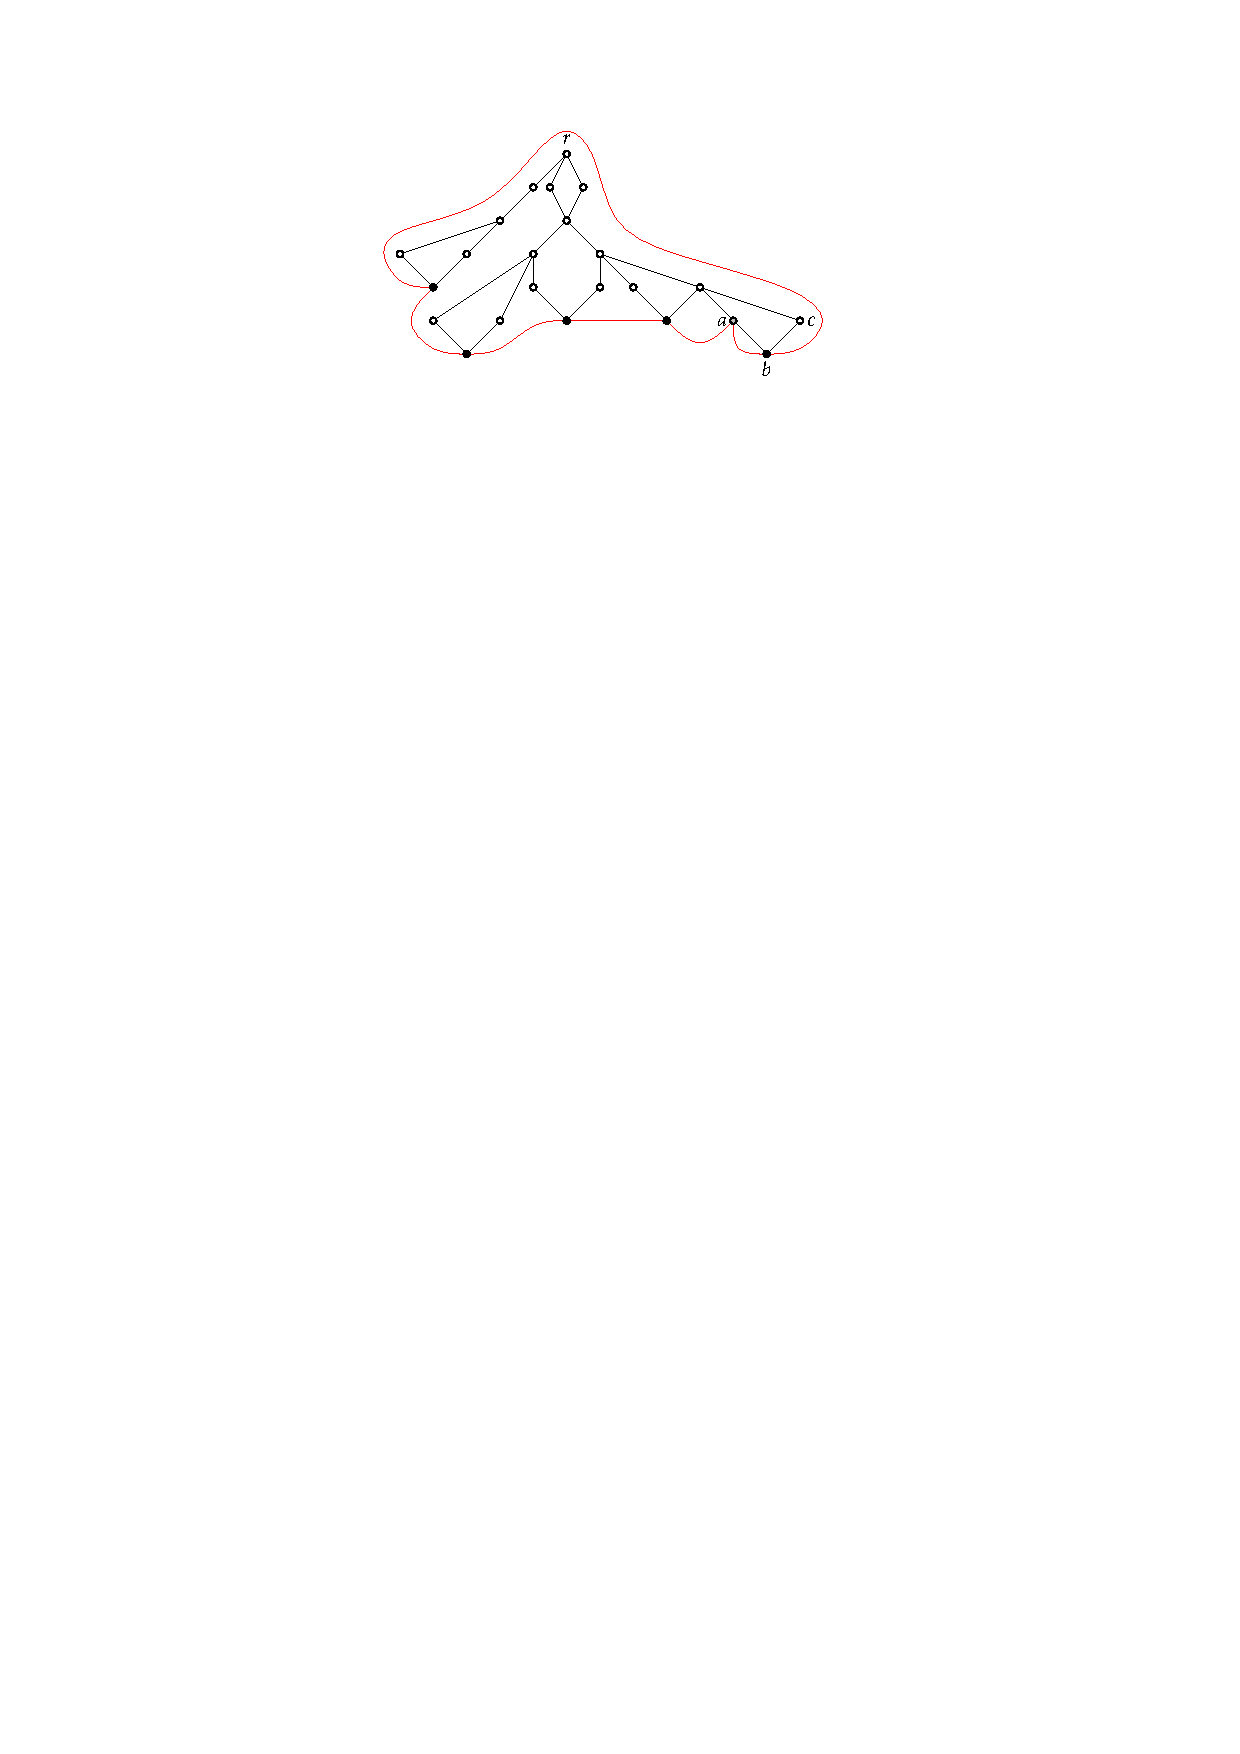
\includegraphics{figs/cactus}
    \end{center}
    \caption{The graph $H$ obtained from a cactus graph with no odd cycles.
        The vertex $a$ is added in the final step so that $H$ is not a cycle
        of length 5.}
    \figlabel{cactus-example}
 \end{figure}

If $\deg_G(r)\ne 1$, there must exist at least one face $F^*$ of $G$ such
that exactly one vertex $v$ of $F^*$ has degree greater than two. From
our choice of $r$, it follows that $\lambda(v)$ is the minimum over all
vertices in $V(F^*)$.  Since $|V(F^*)|\ge 4$, $F^*$ has three consecutive
degree-2 vertices $a$, $b$, and $c$, such that $b\in V(H)$. If $|V(H)|\in
\{5,7,10,14,17\}$, we add $a$ to $V(H)$. If $|V(H)|=9$, we add both $a$
and $c$ to $V(H)$. Notice that now, either $\deg_G(r)=1$ or $|V(H)|\notin
\{5,7,9,10,14,17\}$.

We now define the edge set $E(H)$ of $H$.  For each $u,v\in V(H)$,
we add the edge $uv$ to $E(H)$ if there is a facial path on the outer
face of $G$ with endpoints $u$ and $v$ that does not contain any other
vertices in $V(H)$.  Note that $H$ is either a cycle or a forest of
paths. It can only be a cycle if $G$ has no vertices of degree 1,
in which case, $\deg_G(r)\neq 1$.  In this case, our choice of $V(H)$
ensures that the length of this cycle is not in  $\{5,7,9,10,14,17\}$.
This implies that $H$ can be nonrepetitively coloured using the colour set
$\mathcal{B}=\{1,2,3\}$, either by using the result of Thue \cite{thue1906uber}
or Currie (\thmref{cycle}).

To colour the remaining vertices of $G$, let $h=\max_{v \in V(G)}
\lambda(v)$ and $S=s_0,s_1,\ldots,s_h$ be a palindrome-free nonrepetitive
sequence on $\mathcal{A}=\{4,5,6,7\}$.  Then, each vertex $v\in
V(G)\setminus V(H)$ is assigned the colour $s_{\lambda(v)}$.

We will now show that the resulting 7-colouring of $G$ is a facial
nonrepetitive colouring. Suppose that this is not the case. Thus,
there exists a path $P=P_1,P_2$ such that the colour sequence $S$
corresponding to vertices of $P$ is a repetition. Let us first suppose
that $P$ is on the outer face of $G$. We will need the following claim:

 \begin{clm}\clmlabel{strictly_inc_dec}
  Let $P$ be a path on the outer face of $G$ such that $V(P) \cap V(H) = \emptyset$. The level sequence $L$ corresponding to vertices of $P$ must be strictly decreasing, strictly increasing, or strictly decreasing then strictly increasing.
 \end{clm}
 \begin{proof}[Proof of \clmref{strictly_inc_dec}]
 Suppose that this is not the case. Then $L$ cannot contain two
 consecutive elements of the form $i,i$ as this can only correspond to
 an odd cycle of $G$, but all cycles of $G$ are even. Thus, $L$ must
 contain a block of the form $i,i+1,i$. Since $P$ is on the outer face,
 we must have that the vertex $v$ corresponding to $i+1$ is the lowest
 vertex on some cycle $C$ and that $\deg_G(v)=2$. But in this case, $v$
 must be in $H$, which is a contradiction.
 \end{proof}
 By Lemma \ref{lem:level_pattern_palindrome_free}, $P_1$ and $P_2$ have
 the same level pattern. However, if $V(P) \cap V(H) = \emptyset$ this
 is incompatible with \clmref{strictly_inc_dec}.  Thus, $P$ must contain
 vertices of $H$. Let $P_H=p_1,p_2,\ldots,p_k$ be the sequence of vertices
 of $V(P) \cap V(H)$ in the same order as in $P$. Notice that $P_H$ is
 a path in $H$.  Therefore, the colour sequence corresponding to $P_H$
 is nonrepetitive.  Now, observe that the colour sequence formed by $P$
 is of the form $A_0,B_1,A_1,B_\ell,A_\ell$ where $B_1,\ldots,B_\ell$
 is a non-repetitive sequence of colours from $\mathcal{B}=\{1,2,3\}$ and
 each $A_i$ is a non-repetitive sequence of colours from $\mathcal{A}=\{4,5,6,7\}$.
 Therefore, by \lemref{interleave}, $P$ is coloured nonrepetitively.

Thus, $P$ must be a facial path on some inner face $F$ of $G$.  If $V(P) \cap V(H) =
\emptyset$ then, by Lemma \ref{lem:level_pattern_palindrome_free},
$P_1$ and $P_2$ have the same level pattern.  No path on an even cycle
has such a pattern using the levelling $\lambda$.
Therefore, $V(P)\cap V(H)\neq\emptyset$, so $P$ contains 1, 2, or
3 vertices of $H$.  If $P$ is a repetition it must contain exactly
2 vertices of $H$, thus $P$ is a facial path on $F^*$ (since every
other inner face contributes at most one vertex to $V(H)$).  Reusing the
notation above, $P$ cannot contain $b$ since $b$ has a unique colour in
$V(F^*)$. Therefore, $P$ must contain $a$ and $c$ and, in fact, these are
the endpoints of $P$.  The colour sequence of $P$ must therefore be of
the form $xAx$ where $x\in\{1,2,3\}$ and $A$ is a non-empty sequence over
the alphabet $\{5,6,7,8\}$.  Such a sequence is clearly not a repetition.
\end{proof}


\subsection{Making an Even Blocking Graph}
\seclabel{even-blocking-graph}

\begin{lem}\lemlabel{even-biconnected}
  For every biconnected outerplane graph, $G$, and any vertex $v\in V(G)$:
  \begin{itemize}
    \item $G$ has a blocking set $B$ such that $\block_B(G)$ is an even cycle 
       and $v\in B$; and
    \item $G$ has a blocking set $B$ such that $\block_B(G)$ is an even cycle 
       and $v\not\in B$.
  \end{itemize}
\end{lem}

\begin{proof}
  We first obtain a blocking set $B'$ that contains or does not
  contain $v$, as appropriate, by applying \lemref{biconnected} or
  \corref{biconnected-out}. It is simple to verify that $\block_{B'}(G)$
  is a cycle;  if it is an even cycle, then we are done, so we may assume
  that $\block_{B'}(G)$ is an odd cycle.

  If $G$ has only one inner face, then $B'$ contains one vertex,
  $u$, on this face and $\block_{B'}(G)$ is an odd cycle (of length 1).
  In this case, we can select the neighbour, $w$, of $u$ such that
  $w\neq v$ and let $B=B'\cup\{w\}$.  It is easy to verify that $B$ is
  a blocking set, and either includes or excludes $v$, as appropriate,
  and that $\block_B(G)$ is a 2-cycle.

  Thus, we may assume that $G$ has at least two inner faces and we
  consider several cases:
 
  \begin{enumerate}
  \item If $G$ contains an ear, $F$, with four or more vertices such
  that either $v\not\in V(F)$ or $v$ is one of the endpoints of the
  chord of $F$. There is exactly one vertex $x\in B'$ on the face $F$.
  Let $y$ be a neighbour of $x$ such $y$ is not on the chord of $F$
  (so $y$ has degree 2). Such a $y$ exists since $F$ has at least four
  vertices.  Set $B=B'\cup \{y\}$.  Now $|B|$ is even, so $\block_B(G)$
  is an even cycle.  Furthermore, $G-B'$ is a tree and $y$
  is a leaf in this tree, so $G-B$ is also a tree.  Finally,
  by choice, $B$ contains $v$ if and only if $B'$ contains $v$, so $B$
  satisifies the conditions of the lemma.

  \item Next, consider the case where $G$ contains triangular ear, $F$,
  such that one of the endpoints of the chord of $F$ is in $B'$ and $v$
  is not the degree 2 vertex, $y$, of $F$.  By the same argument as above,
  $B=B'\cup\{y\}$ satisfies the conditions of the lemma, so we are done.

  \item Refer to \figref{toughie}. 
  For an edge $uw\in E(G)$, let $V_{uw}'$ and $V_{uw}''$ be the two
  (possibly empty) sets of vertices in the two connected components
  of $G-\{u,w\}$.  Let $G_{uw}'=G[V_{uw}'\cup\{u,w\}]$ and
  $G_{uw}''=G[V_{uw}''\cup\{u,w\}]$.

  \begin{figure}
    \begin{center}
       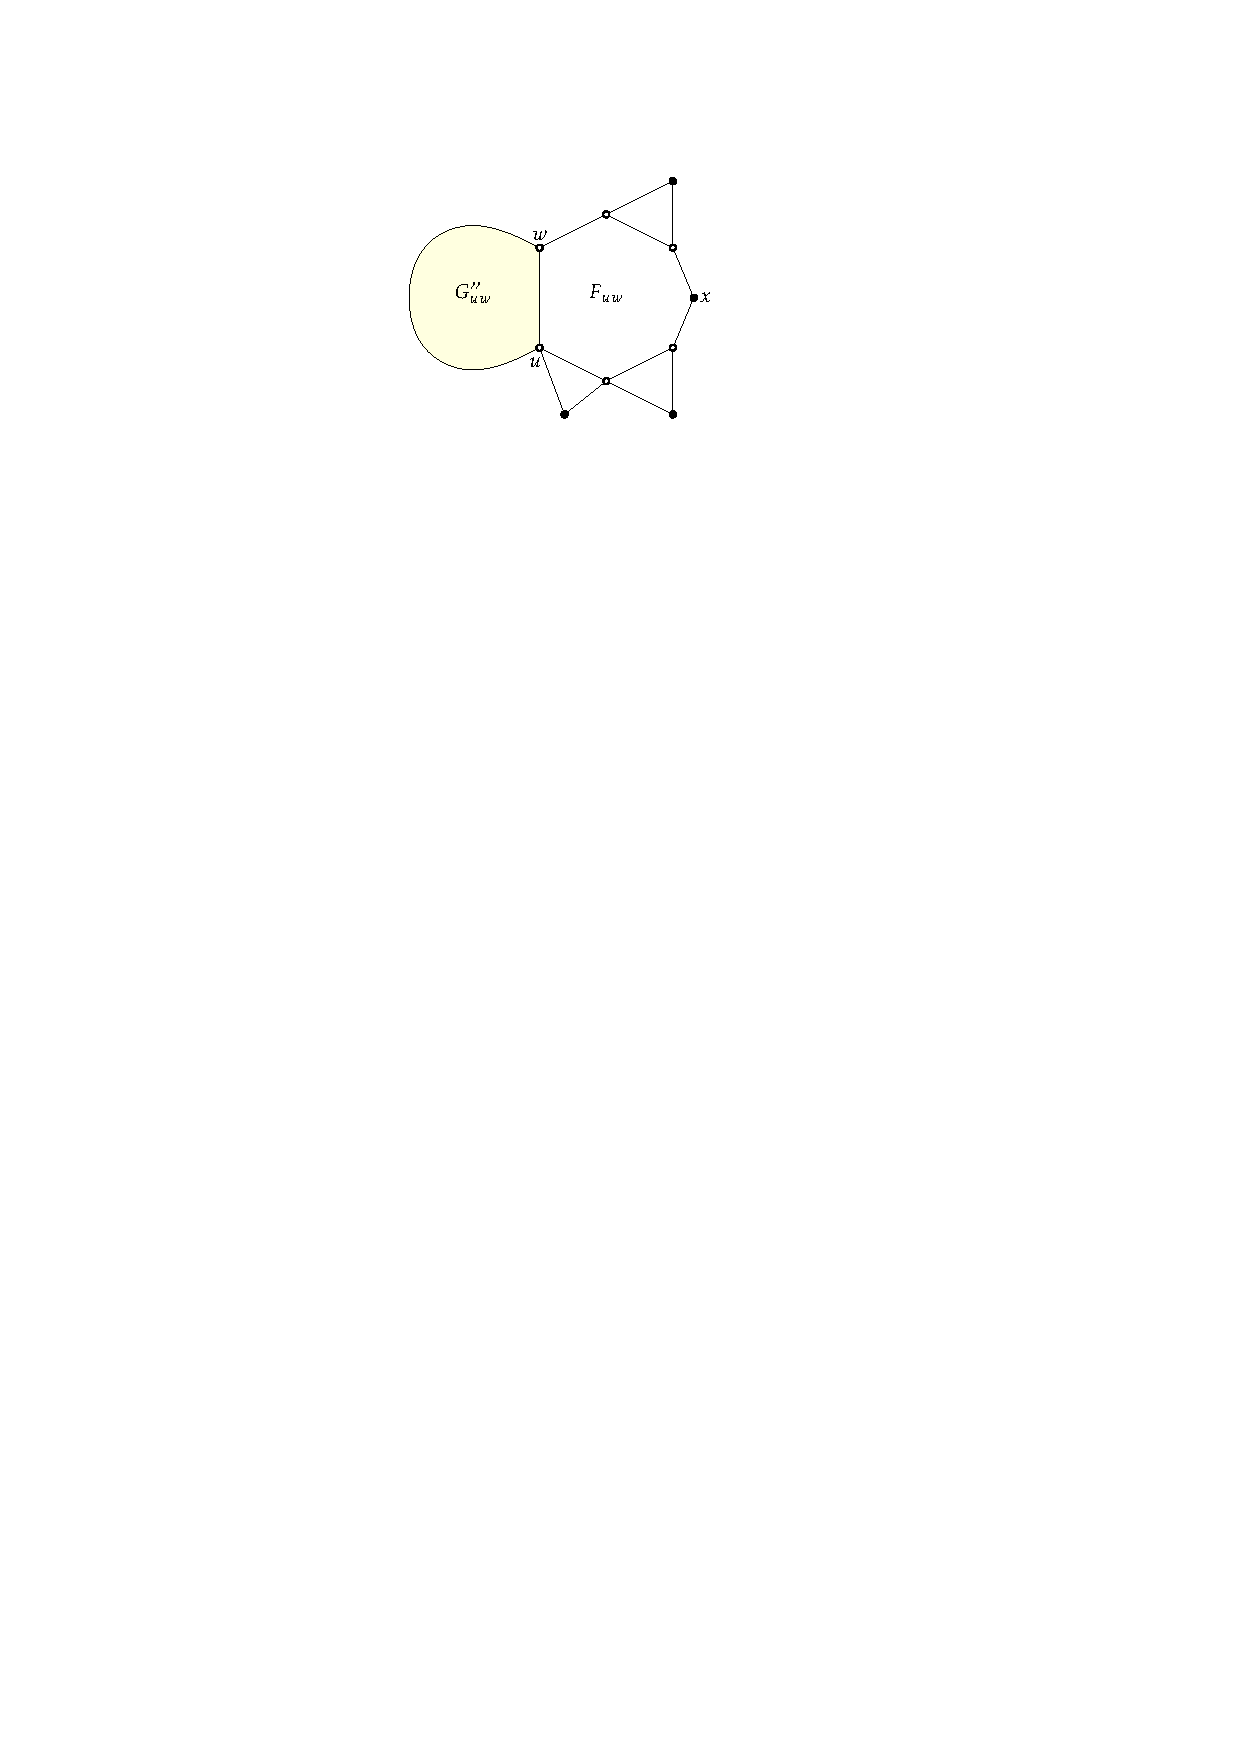
\includegraphics{figs/toughie}
    \end{center}
    \caption{The face $F_{uw}''$ in the proof of \lemref{even-biconnected}.}
    \figlabel{toughie}
  \end{figure}

  If neither of the two previous cases applies, then there exists an edge
  $uw$ of $G$ such that $v\not\in V_{uw}'$ and the weak dual of $G_{uw}'$
  is a star whose central vertex is the face, $F_{uw}$ incident on $uw$.
  (Note that $v$ may be one of $u$ or $w$.)

  We will now show that we can select another vertex, $y$, from
  $V_{uw}'\setminus B'$ so that $B=B'\cup\{y\}$ is a blocking set.
  This is sufficient since $|B|$ is even so $\block_B(G)$ is an even
  cycle.  

  \begin{itemize}
  \item[$(\star)$]
  By choice, $G_{uw}'$ has at least 2 faces and each of them, other
  than $F_{uw}$, is a triangular ear incident to $F_{uw}$ and whose
  degree-2 vertex is in $B'$ (otherwise, one of those faces would have
  been handled by Case~1 or 2).
  \end{itemize}

  Let $x$ be the unique vertex of $B'$ on $F_{uw}$. The vertex $x$ has two
  neighbours on $F_{uw}$.  We claim that one of these is not in $\{u,w\}$
  and we take this vertex to be $y$.  This claim is valid because
  otherwise, $F_{uw}$ is a triangle, $xuw$, with $x\not\in\{u,w\}$.
  This case is not possible because by $(\star)$ at least one of $xu$ or
  $xw$ is incident on both $F_{uw}$ and a triangular ear $E$ of $G_{uw}'$.
  Both $x$ and the degree 2 vertex of $E$ are in $B'$.  This contradicts
  the fact that $B'$ includes at most one vertex from each face of $G$,
  including $E$.

  Let $B=B'\cup\{y\}$.  We claim that $B$ is a blocking set of $G$.
  First, note that $B$ contains at most two vertices from each face, $F$,
  of $G$, so $V(F)\setminus B'\neq \emptyset$.  We now show that $y$ is a
  leaf in the tree $G-B'$, so that $G-B$ is also a tree.

  First, observe that $xy$ is not a chord of $G$ since, by $(\star)$,
  the face incident to $xy$ other than $F_{uw}$ would have two of its
  vertices in $B'$.  Thus, in addition to $x$, $y$ has at most two
  neighbours in $G$.  One of these, $z$, is on $F_{uw}$ and $z\neq x$
  so $z\notin B'$.  Finally, $y$ may have one additional neighbour,
  which is a degree-2 vertex of a triangular ear incident on $yz$.
  In this case, by $(\star)$, this degree-2 vertex is in $B'$.  Thus,
  $yz$ is the only edge incident to $y$ in the tree $G-B'$
  so $y$ is a leaf in this tree. \qedhere
\end{enumerate}
\end{proof}

\begin{rem}\remlabel{bw}
   The proof of \lemref{even-biconnected} can be modified to prove
   something stronger than just requiring the inclusion or exclusion
   of $v\in B$.  We can specify an edge $ab$ on the outer face of $G$
   and obtain a blocking set $B$ such that $\block_B(G)$ is an even
   cycle, $a\not\in B$ and $b\in B$.  The only difference in the proof
   is ensuring that $a$ is not included in $B$. The resulting proof
   has the same three cases. Case~1 applies as long as $ab$ is not on
   the boundary of the ear $F$. Case~2 applies as long as $ab$ is not
   on the boundary of the ear $E$.  Otherwise, in Case~3, the edge $ab$
   is in the subgraph $G_{uw}''$, so there is no chance of including $a$
   in $B$.  This stronger version of \lemref{even-biconnected} is used
   in \appref{biconnected}.
\end{rem}

\begin{lem}\lemlabel{even-bridgeless}
  Every simple bridgeless outerplane graph $G$ has a blocking set $B$
  such that all cycles in $\block_B(G)$ are even.
\end{lem}

\begin{proof}
  The proof is by induction on the number of 2-connected components
  of $G$.  If $G$ has no 2-connected components, then we take $B$ to be
  the empty blocking set.  If $G$ has only one 2-connected component,
  then we apply \lemref{even-biconnected}.
  Otherwise, select a 2-connected component, $C$, that
  shares exactly one vertex, $v$, with the rest of $G$.  Let
  $G'=G-(V(C)\setminus\{v\})$ and apply induction on $G'$
  to obtain a blocking set, $B'$, of $G'$ such that $\block_{B'}(G')$
  has only even cycles.  There are two cases to consider:
  \begin{enumerate}
    \item If $B'$ contains $v$, then we apply the first part of
    \lemref{even-biconnected} to obtain a blocking set $B''$ of $C$
    such that $\block_{B''}(C)$ is an even cycle and $v\in B''$.  We take
    $B=B'\cup B''$, which clearly forms a blocking set of $G$.  
    The blocking graph $\block_B(G)$ is simply the union of the
    two blocking graphs $\block_{B'}(G)$ and $\block_{B''}(C)$, which have
    only the vertex $v$ in common.  Thus, every cycle in $\block_B(G)$
    is also a cycle in one of these two graphs, so it has even length.

    \item If $B'$ does not contain $v$, then we apply the second part
    of \lemref{even-biconnected} to obtain a blocking set $B''$ of $C$
    such that $\block_{B''}(C)$ is an even cycle and $v\not\in B''$.
    We take $B=B'\cup B''$.

    Refer to \figref{block-merge}.  
    Starting at some appropriate vertex in $V(G)\setminus V(C)$
    in the facial walk on the outer face of $G$, there is a last vertex,
    $x\in V(G')\cap B'$, encountered before the walk encounters the first
    vertex $u\in V(C)\cap B''$ and there is a last vertex $w\in V(C)\cap
    B''$ encountered before the walk returns to the next vertex $y\in
    V(G')\cap B'$.  The edge $xy$ is in $\block_{B'}(G')$ and the edge
    $vw$ is in $\block_{B''}(C)$.

    \begin{figure}
       \begin{center}
         \begin{tabular}{m{.45\textwidth}m{.05\textwidth}m{.45\textwidth}}
          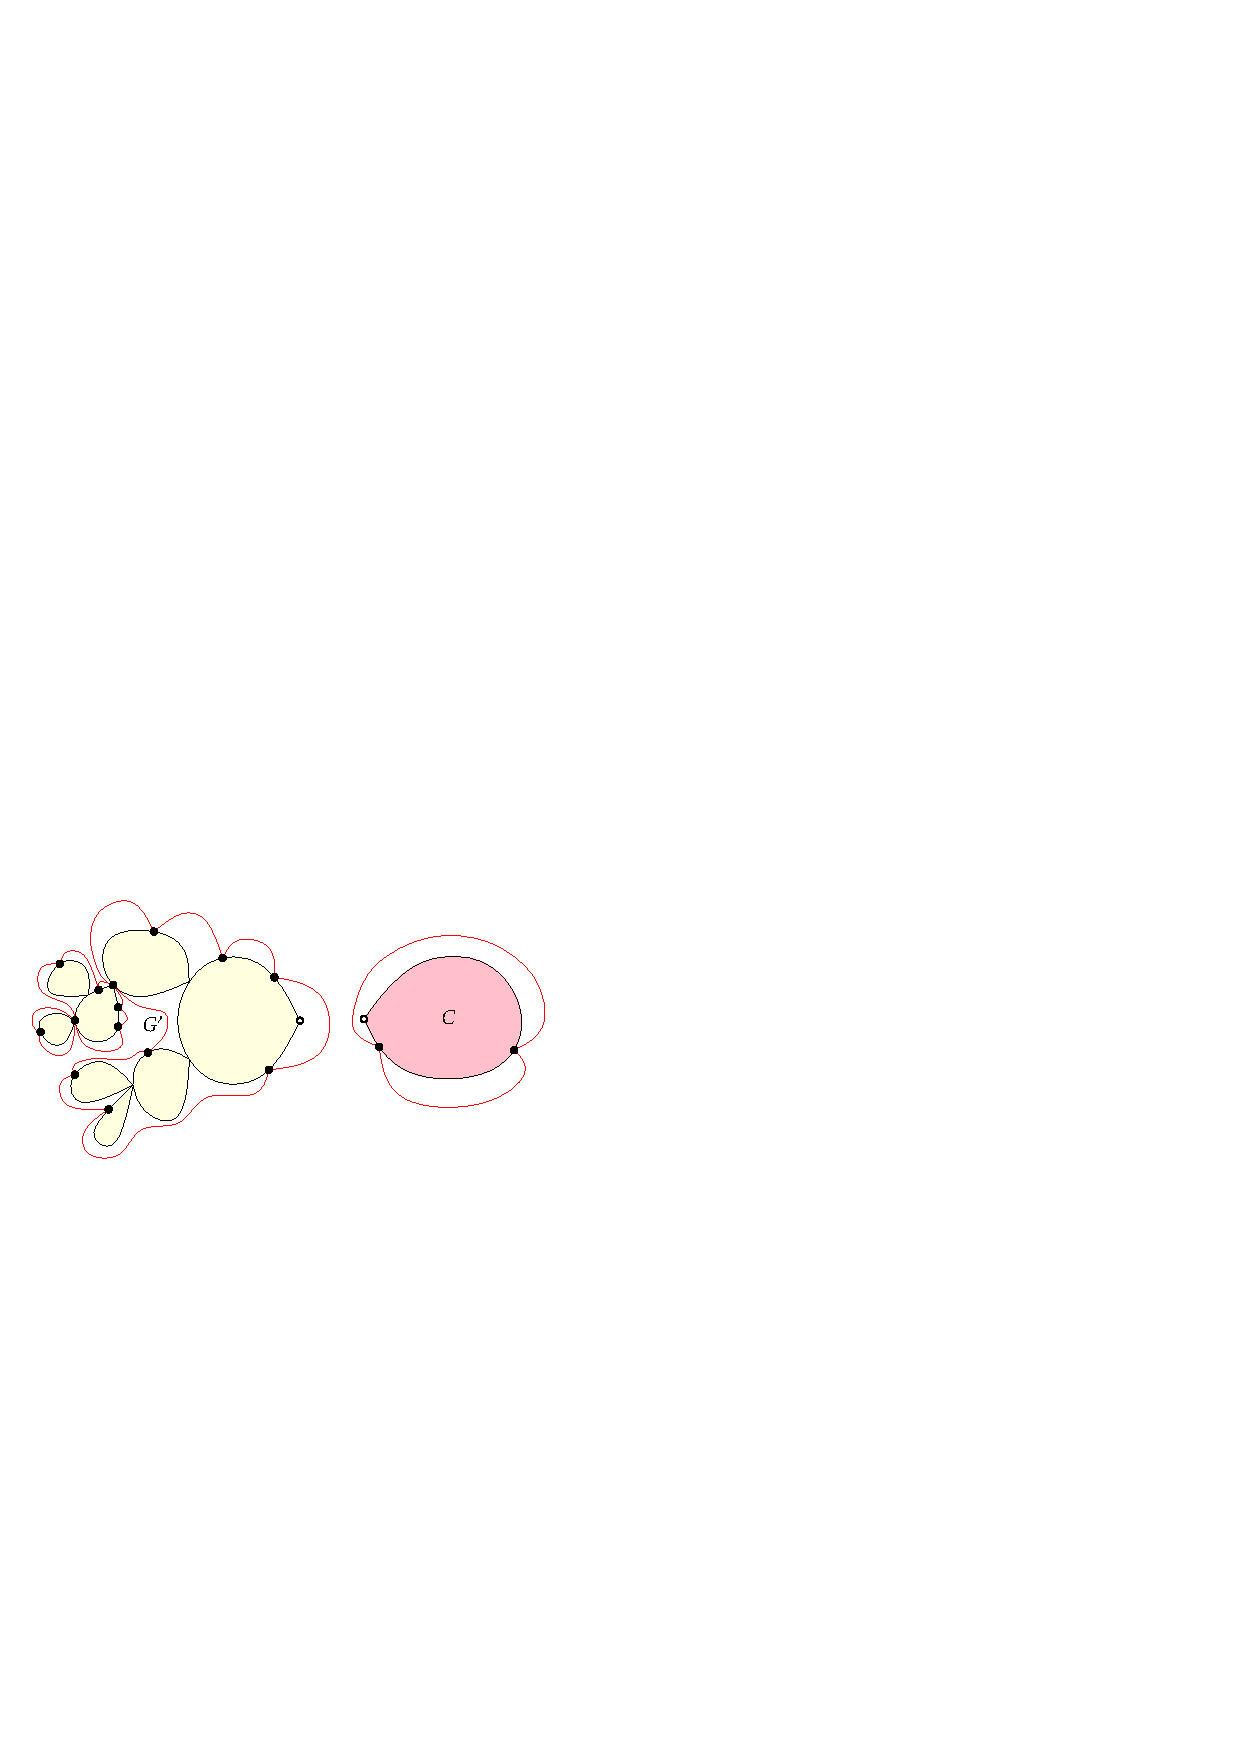
\includegraphics[width=.45\textwidth]{figs/good-one-1} &
          $\Rightarrow$ &
          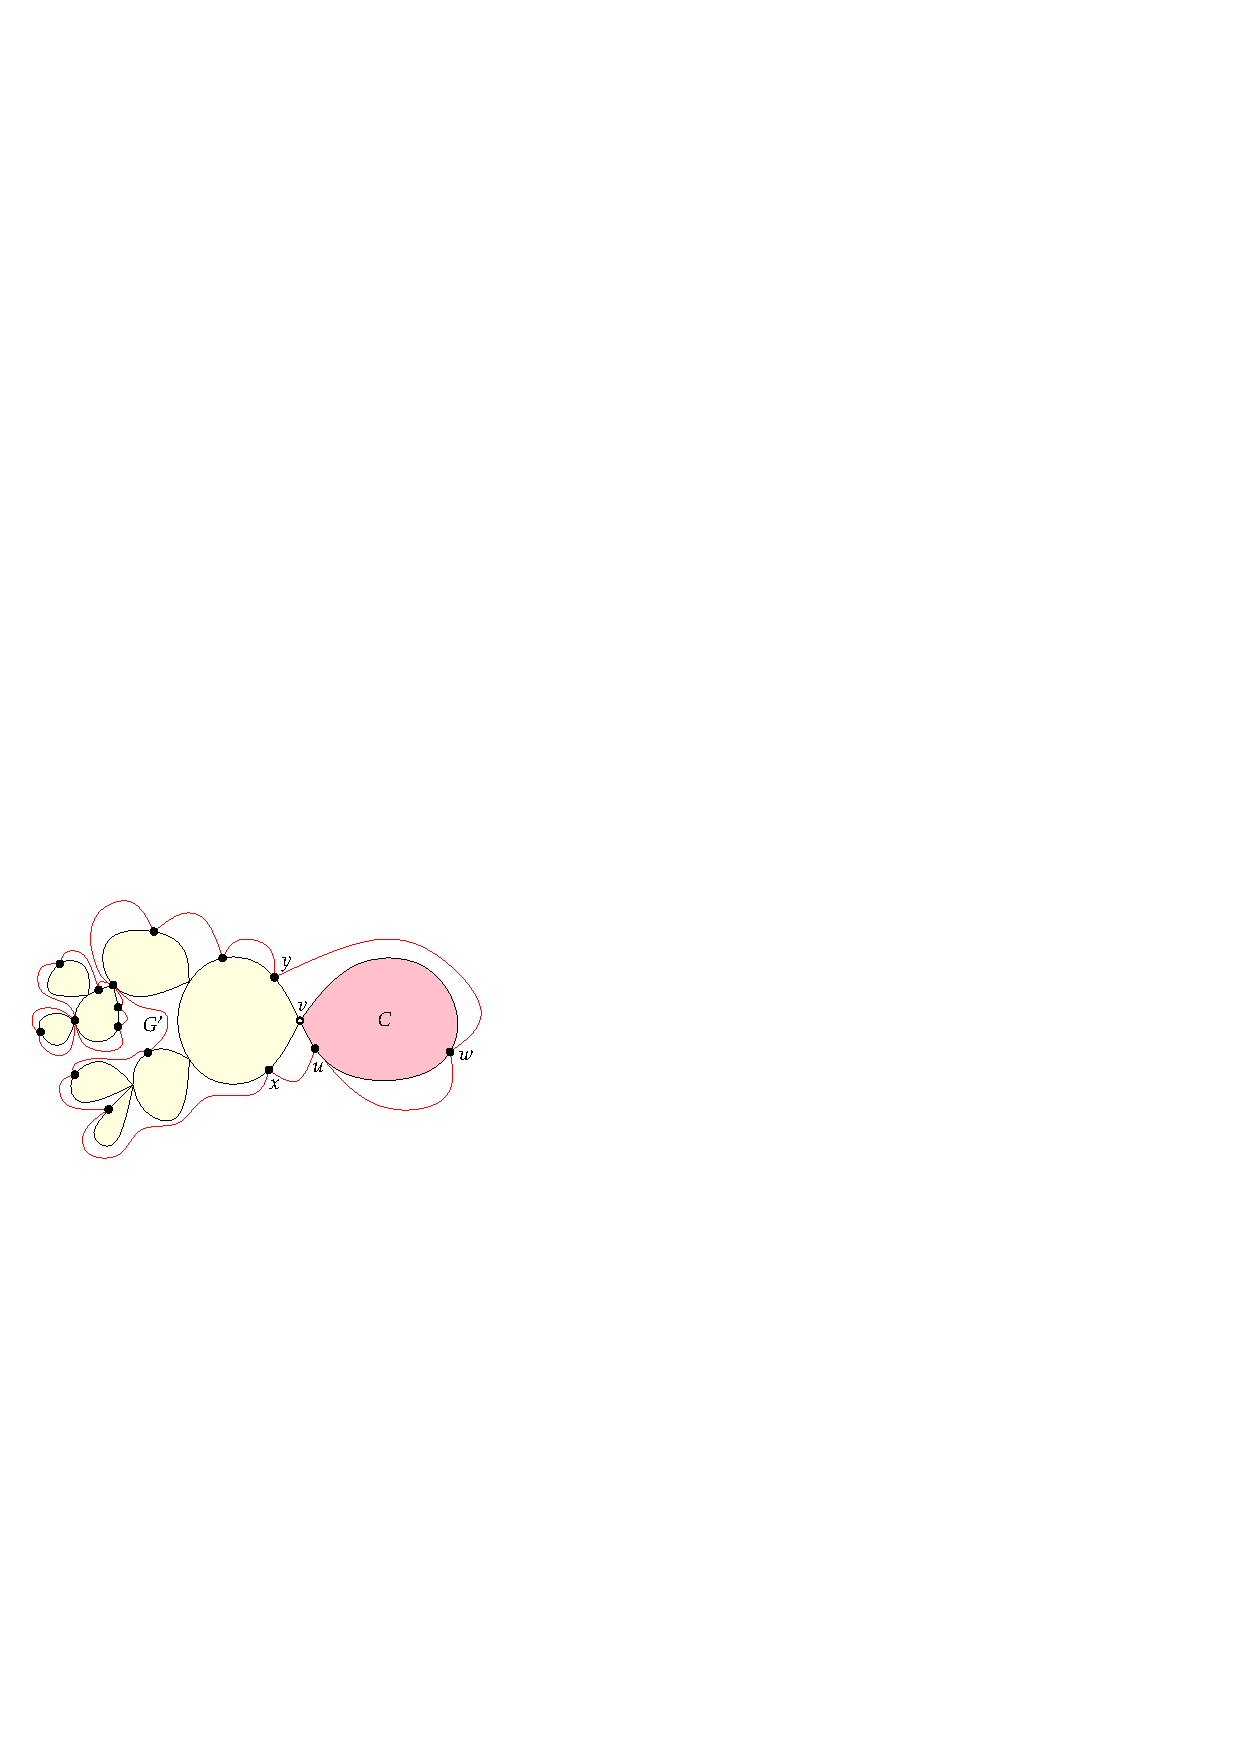
\includegraphics[width=.45\textwidth]{figs/good-one-2}
         \end{tabular}
       \end{center}
       \caption{Case~2 in the proof of \lemref{even-bridgeless}.}
       \figlabel{block-merge}
    \end{figure}

    Since every blocking graph is a bridgeless cactus graph
    (\obsref{cactus}), each of these edges is part of one even cycle
    in its respective graph. In $\block_{B}(G)$ these two cycles are
    merged by removing the edges $xy$ and $vw$ and adding the edges
    $xv$ and $yw$.  The resulting cycle is even.  Every other cycle
    in $\block_B(G)$ is also a cycle in one of $\block_{B'}(G')$ or
    $\block_{B''}(C)$ so it has even length. \qedhere
  \end{enumerate}
\end{proof}

\begin{lem}\lemlabel{even}
  Every simple outerplane graph $G$ has a blocking set $B$ such that
  all cycles in $\block_B(G)$ are even.
\end{lem}

\begin{proof}
  The proof is by induction on the number of bridges of $G$.  If $G$
  has no bridges, then we apply \lemref{even-bridgeless}.  Otherwise,
  select some bridge $uw$ of $G$ and contract it to obtain a graph $G'$
  in which $uw$ corresponds to a single vertex $v$.  By induction,
  we obtain a blocking set $B'$ of $G'$ such that $\block_{B'}(G')$
  has only even cycles (or is empty).  There are two cases to consider:
  \begin{enumerate}
    \item If $v\in B'$, then we take $B=B'\cup\{u,w\}\setminus\{v\}$. This introduces exactly one new cycle in $\block_B(G)$ that is not present in $\block_{B'}(G')$ and this cycle has length 2.

    \item If $v\not\in B'$, then we take $B=B'$, so
    $\block_B(G)=\block_{B'}(G')$. \qedhere
  \end{enumerate}
\end{proof}

Finally, have all the tools to prove our main result on outerplane graphs:

\begin{thm}\thmlabel{outerplane}
  For every outerplane graph, $G$, $\pi_f(G)\le 11$.
\end{thm}

\begin{proof}
By \lemref{non-simple}, we may assume that $G$ is simple.  From
\lemref{even}, $G$ has a blocking set $B$ such that $\block_B(G)$
has no odd cycles.  Therefore, by \lemref{cactus}, $\pi_f(\block_B(G))\le
7$.  Using this with \lemref{k-plus-four} implies that $\pi_f(G)\le 11$.
\end{proof}



\section{Plane Graphs}

In this section, we show how to reuse the ideas from Bar\'at and Czap
\cite{barat2013facial} to facially nonrepetitively 22-colour every plane graph.
Some modifications are needed because Bar\'at and Czap use a nonrepetitive
12-colouring of outerplanar graphs whereas our \thmref{outerplane} provides an
nonrepetitive 11-colouring but only for facial paths of outerplane graphs.

\begin{thm}
   Let $r=\max\{\pi_f(G):\text{$G$ is outerplane}\}$.  Then, for every
   plane graph $G$, $\pi_f(G)\le 2r$.
\end{thm}

\begin{proof}
   For any plane graph, $H$, the \emph{peeling layering} of $H$ is
   a partition of $V(H)$ into sets as follows.  Let $V_0(H)$ be the
   vertices on the outer face of $H$ and let $V_i(H)$, $i\ge 1$, be the
   vertices on the outer face of $H-(V_0(H)\cup\cdots\cup V_{i-1}(H))$.

   We augment $G$ to obtain a plane graph $G^+$ in the following way.
   For each inner face $F$ of $G$, let $W$ be the facial walk of $F$.
   The walk $W$ contains only vertices from $V_i(G)$ and $V_{i+1}(G)$
   for some $i$.  Remove from $W$ all vertices in $V_{i+1}(G)$ to
   obtain a cyclic sequence $W'$ of vertices from $V_i(G)$.  For any
   two consecutive vertices $u,w$ in $W'$, we add the edge $uw$
   to $G^+$ and embed it inside the face $F$. This construction has
   the following implications: (a)~The resulting graph $G^+$
   is still plane (though not necessarily simple) and, for all
   $i$, $V_i(G)=V_i(G^+)$. From this point onward, we use the notation
   $V_i=V_i(G)=V_i(G^+)$.
   (b)~The cyclic sequence $W'$ defined above is a facial walk
   in $G^+$ and, since it contains only vertices in $V_i$, it is also
   a facial walk in $G^+[V_i]$.

   For each $i$, $G^+[V_i]$ is outerplane.  To colour $G$ we use
   \thmref{outerplane} to facially nonreptitively colour $G^+[V_i]$ with
   $\{1,\ldots,11\}$ if $i$ is even or $\{12,\ldots,22\}$ if $i$ is odd.
   This defines a colouring of $G$ that we now prove is facially
   nonrepetitive.

   Let $P$ be a facial path, $F$, in $G$. The graphs $G^+[V_0]$ and $G$
   have the same outside face so, if $P$ is on the outside face,
   then the colour sequence of $P$ is not a repetition
   since our colouring is facially nonrepetitive for $G^+[V_0]$.

   Therefore, $F$ is an inner face and all vertices on $F$ are in $V_i\cup
   V_{i+1}$ for some $i$.  Write $P$ as $P_0,Q_1,P_1,\ldots,Q_k,P_k$,
   where each $Q_j$ consists of vertices from $V_i$ and each $P_j$
   consists of vertices from $V_{i+1}$.  Notice that, for each
   $j\in\{1,\ldots,k-1\}$, $G^+[V_i]$ contains an edge joining the
   last vertex in $Q_j$ to the first vertex in $Q_{j+1}$.  Indeed,
   $Q_{1},\ldots,Q_k$ is a facial path in $G^+[V_i]$ (It is a contiguous
   subsequence of the sequence $W'$ defined above.)  Next, observe that
   each $P_j$ is a facial path on the outer face of $G^+[V_{i+1}]$.
   Therefore, the colour sequence determined by $P$ is of the form
   $A_0,B_1,A_1,\ldots,B_k,A_k$ (with $A_j$ corresponding to $P_j$
   and $B_j$ corresponding to $Q_j$).  The sequence $B_1,\ldots,B_k$ is
   nonrepetitive and each sequence $A_j$ is non-repetitive.  Therefore,
   by \lemref{interleave}, the colour sequence determined by $P$
   is nonrepetitive.
\end{proof}

\bibliographystyle{plain}
\bibliography{facial}

\appendix
\section{Biconnected Outerplane Graphs}
\applabel{biconnected}

\begin{lem}\lemlabel{good-one}
  If $G$ is a biconnected outerplane graph, then $G$ has a blocking set $B$
  such that $|B|\not\in\{5,7,9,10,14,17\}$.
\end{lem}

\begin{proof}
  If $G$ is a cycle, take $B$ to be two consecutive vertices on $G$.
  Otherwise, select an ear, $E$ of $G$ and let $uv$ be $E$'s chord.
  Then apply the stronger version of \lemref{even} discussed in
  \remref{bw} to the graph $G'=G-(V(E)\setminus\{u,v\})$ to obtain a
  blocking set $B'$ of even size that contains $v$ and not $u$.

  Note that, since $v\in B'$ and $v$ is on $E$,  $G-B'$ has no cycles.
  Furthermore, since $u\not\in B'$, $G-B'$ is connected, so $B'$
  is a blocking set of $G$.  Since $|B'|$ is even, 
  $|B'|\not\in\{5,7,9,17\}$, so if $|B'|\not\in\{10, 14\}$, then we are
  done with $B=B'$. Otherwise, let $y$ be $v$'s degree-2 neighbour on $E$
  and take $B=B'\cup\{y\}$.
\end{proof}

\begin{cor}
  If $G$ is an outerplane graph with at most one 2-connected component, 
  then $\pi_f(G)\le 7$.
\end{cor}

\begin{proof}
  If $G$ is a tree, then $\pi_f(G)\le 4$, so we may assume $G$ contains
  exactly one 2-connected component, $G'$.  Apply \lemref{good-one} to
  $G'$ to obtain a blocking set $B$ with $|B|\not\in\{5,7,9,10,14,17\}$
  and observe that $B$ is also a blocking set of $G$.  The blocking graph
  $\block_B(G')$ is a cycle, $C$, that has a nonrepetitive 3-coloring.
  The blocking graph $\block_B(G)$ consists of $C$ and possibly some
  self loops so, by \lemref{non-simple}, $\block_B(G)$ has a facial
  nonrepetitive 3-colouring.  Therefore, by \lemref{hitting_plus_four},
  $\pi_f(G)\le 7$.
\end{proof}



\end{document}


